Random Forest là một phương pháp học máy mạnh mẽ, được sử dụng để thực hiện các nhiệm vụ phân loại, hồi quy và nhiều tác vụ khác bằng cách xây dựng nhiều cây quyết định và kết hợp chúng lại thành một "rừng". Mỗi cây quyết định trong rừng được huấn luyện trên một mẫu dữ liệu con được lấy ngẫu nhiên từ tập dữ liệu gốc và sử dụng một tập con ngẫu nhiên của các thuộc tính tại mỗi nút để đưa ra dự đoán.

\begin{figure}[htbp]
\centerline{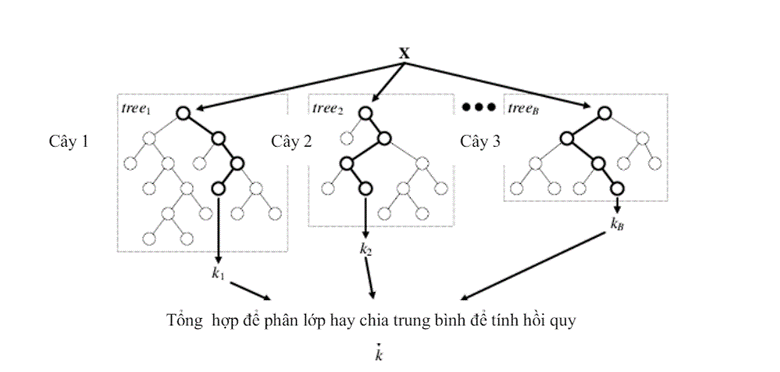
\includegraphics[width=0.4\textwidth]{img/RF.png}}
\caption{Sơ đồ biểu diễn các cây quyết định trong Random Forest}
\label{fig}
\end{figure}

Mỗi node trong của cây quyết định đại diện cho một thuộc tính, và các nhánh biểu thị các giá trị có thể của thuộc tính đó. Bằng cách đi từ gốc đến các node của cây theo các giá trị thuộc tính, cây quyết định có thể dự đoán giá trị đầu ra cho một đối tượng. Điểm mạnh của nhóm thuật toán cây quyết định là khả năng áp dụng vào các bài toán phân loại và hồi quy. Vì vậy, Random Forest có thể được sử dụng để phân tích và dự báo chuỗi thời gian. Random Forest cũng có khả năng đánh giá tầm quan trọng của các thuộc tính, giúp chúng ta hiểu rõ hơn về ảnh hưởng của từng thuộc tính đến kết quả dự đoán. Từ hình trên, ta có thể thấy rằng Random Forest bao gồm nhiều cây quyết định. Khi nhận đầu vào là một đối tượng x, mỗi cây sẽ đưa ra dự đoán riêng về giá trị của biến mục tiêu. Những dự đoán này sau đó được tổng hợp lại bằng cách lấy trung bình để đưa ra quyết định cuối cùng của mô hình.


